\section{The Derivative}
\label{sec:derivative}

\subsection{Derivative Concepts and Notation}

\begin{definition}
We can view the {\bf derivative}\index{Derivative} of a function, $f(x)$ in several different equivalent ways. Here are three of them. The derivative of $f(x)$ at a point $(a, f(a))$ is:
    \begin{itemize}
    \item the instantaneous rate of change of $f(x)$ at $x=a$, 
    \item the slope of the tangent line to the graph of $f(x)$ at the point $(a,f(a))$, and
    \item the slope of the curve $y=f(x)$ at the point $(a,f(a))$.
    \end{itemize}
\end{definition}

We've been acting as if derivatives exist everywhere for every function. This is true for most of the functions that you will run into in this textbook. But there are some common places where the derivative doesn't exist.

\begin{definition}
A function, $f(x)$, is called {\bf differentiable}\index{Differentiable} at the point $(a,f(a))$ if its derivative exists at $x=a$.
\end{definition}

Remember that the derivative is the slope of the tangent line to the curve. That's what to think about.

Where can a slope not exist? If the tangent line is vertical, the derivative will not exist.

\begin{example}
Show that $f(x)=\sqrt[3]{x}=x^{1/3}$ is not differentiable at $x=0$.

\begin{solution} From the graph in Figure \ref{fig:2-3-cuberoot}, we can see that the tangent line to $y=\sqrt[3]{x}$ at $x=0$ is vertical with undefined slope, which is why the derivative does not exist at $x=0$.

\begin{figure}[!ht]
  \centering
    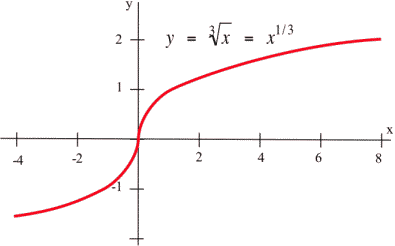
\includegraphics[width=0.4\textwidth]{img/chap2/image037.png}
    \caption{$f(x)=\sqrt[3]{x}$}
    \label{fig:2-3-cuberoot}
\end{figure}
\end{solution}\end{example}

Where can a tangent line not exist?

If there is a sharp corner (cusp)\index{Cusp} in the graph, the derivative will not exist at that point because there is no well-defined tangent line (a teetering tangent, if you will).

If there is a discontinuity\index{Discontinuity} in the graph (a jump, a break, a hole in the graph, or a vertical asymptote), the tangent line will be different on either side and the derivative will not exist at that point.

\begin{example}
Show that $f(x)=|x|$ is not differentiable at $x=0$.

\begin{solution} On the left side of the graph in Figure \ref{fig:2-3-absx}, the slope of the line is $-1$. On the right side of the graph, the slope is $1$. There is no well-defined tangent line at the sharp corner at $x=0$, so the function $|x|$ is not differentiable at that point.

\begin{figure}[!ht]
  \centering
    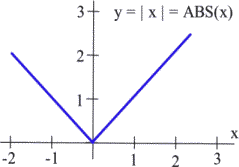
\includegraphics[width=0.4\textwidth]{img/chap2/image038.png}
    \caption{$f(x)=|x|$}
    \label{fig:2-3-absx}
\end{figure}
\end{solution}\end{example}


\begin{definition}
When we find the derivative of a function, or take the derivative of a function, we say that we {\bf differentiate}\index{Differentiate} the function.
\end{definition}

\paragraph*{Notation for the Derivative}
Calculus was invented by Leibniz\index{Leibniz, Gottfried} and Newton\index{Newton, Isaac}, but it was developed by many more throughout the subsequent centuries. Many developed their own notation for the derivative of a function. The notation developed by Leibniz and Joseph-Louis Lagrange\index{Lagrange, Joseph-Louis} are the most convenient and most used. 

The derivative of $y=f(x)$, with respect to $x$, is written in many different ways:
\begin{itemize}
    \item $f'(x)$: ``$f$ prime of $x$'',
    \item $y'$: ``$y$ prime,''
    \item $\dfrac{dy}{dx}$: ``$d$ $y$ $d$ $x$,''  
    \item $\dfrac{df}{dx}$: ``$d$ $f$ $d$ $x$,'' or
    \item $\dfrac{d}{dx}f(x)$: ``$d$ $d$ $x$ of $f$ of $x$.''
\end{itemize}
The notation that resembles a fraction is called {\bf Leibniz notation}\index{Leibniz notation}. It displays not only the name of the function ($f$ or $y$), but also the name of the variable (in this case, $x$). It looks like a fraction because the derivative is a slope. In fact, this is simply $\dfrac{\Delta y}{\Delta x}$ written in Roman letters instead of Greek letters. The nuance here is that $\Delta v$\index{Delta} represents a finite difference of some variable $v$, whereas $dv$ represents an {\bf infinitesimal}\index{Infinitesimal} difference of a variable $v$. An infinitesimal difference would be a difference that is infinitely small, but not 0. That may sound like an oxymoron, but until about 1850, calculus was developed using infinitesimal differences, also called {\bf differentials}\index{Differential}. 

The best way to understand differentials is with an analogy: $1:\infty::dx:1$. Suppose you had a bin with an infinite number of balls and you throw one ball in. You still throw in a ball, but the total quantity of balls in the bin is unchanged. In the same way, if you have a line that is one inch long and you add on a line of length $dx$ inches, then the line is still one inch long, despite ``lengthening'' the line by $dx$.
 
\paragraph*{Looking Ahead}
We will figure out ways to compute exact values of derivatives from many kinds of functions in Sections \ref{sec:algderiv}-\ref{sec:chain}. If the function is given to you as a table or graph, you will still need to approximate the derivative of the function this way.

This is the foundation for the rest of this chapter. It's remarkable that such a simple idea (the slope of a tangent line) and such a simple definition (for the derivative $f'(x)$) will lead to so many important ideas and applications.

\subsection{The Derivative as a Function}
We now know how to find (or at least approximate) the derivative of a function for any $x$-value. This means that we can think of the derivative as a function too. That is the origin of the term ``derivative.'' The derivative of a function is a function that is derived from that function. The input of the derivative is the same as the function, but the output is the value of the derivative at that $x$ value and the units reflect the rate of change concept.

\begin{example}
Below is the graph of a function $y=f(x)$. We can use the information in the graph to fill in a table showing values of $f'(x)$:
\begin{figure}[!ht]
  \centering
    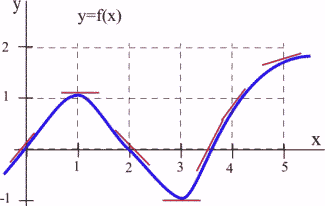
\includegraphics[width=0.4\textwidth]{img/chap2/image023.png}
    \caption{$y=f(x)$}
    \label{fig:2-3-fx}
\end{figure}

\begin{solution} At various values of $x$, draw your best guess at the tangent line and measure its slope. You might have to extend your lines so you can read some points. In general, your estimate of the slope will be better if you choose points that are easy to read and far away from each other. Here are estimates for a few values of $x$ (parts of the tangent lines used are shown above in the graph):
\begin{table}[ht!]
\begin{centering}
\begin{tabular}{ccc}
\toprule
$x$ &   $y=f(x)$    &	$f'(x)$\\
\midrule
0   &	0 &	1	\\
1   &	1 &	0	\\
2   &	0 &	$-1$  \\
3   &  $-1$ &	0	\\
3.5 &	0 &	2   \\
\bottomrule
\end{tabular}
\caption{Table of inputs, outputs, and derivatives of $f(x)$.}
\label{tab:2-3-deriv}
\end{centering}
\end{table}
Based on this, we can estimate the values of $f'(x)$ at some non-integer values of $x$ too: $f'(0.5)\approx   0.5$ and $f'(1.3)\approx   -0.3$.
\begin{figure}[!ht]
  \centering
    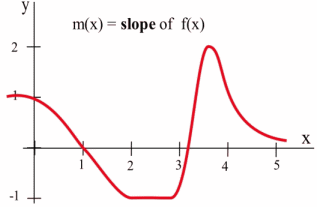
\includegraphics[width=0.4\textwidth]{img/chap2/image024.png}
    \caption{Slope of $y=f(x)$}
    \label{fig:2-3-fprimex}
\end{figure}
We can even think about entire intervals. For example, if $0<x<1$, then $f(x)$ is increasing; all the slopes are positive, and so $f'(x)>0$.

The values of $f'(x)$ definitely depend on the values of $x$, and $f'(x)$ is a function of $x$. We can use the results in the table to help sketch the graph of $f'(x)$.

\end{solution}\end{example}
\begin{example}
Figure \ref{fig:2-3-ht} shows the graph of the height, $h(t)$, of a rocket $t$ seconds after liftoff.

\begin{figure}[!ht]
  \centering
    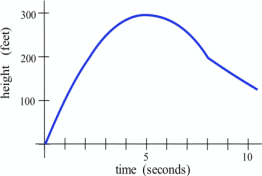
\includegraphics[width=0.4\textwidth]{img/chap2/image025.png}
    \caption{$y=h(t)$}
    \label{fig:2-3-ht}
\end{figure}
Sketch the graph of the velocity of the rocket at time $t$. (Velocity is the derivative of the height function, so it is the slope of the tangent to the graph of position or height.)

\begin{solution} We can estimate the slope of the function at several points. The graph in Figure \ref{fig:2-3-hprime} shows the velocity of the rocket. This is $v(t)=h'(t)$.

\begin{figure}[!ht]
  \centering
    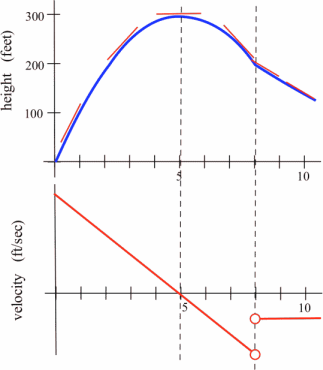
\includegraphics[width=0.4\textwidth]{img/chap2/image026.png}
    \caption{$y=h(x)$ and $y=h'(x)$}
    \label{fig:2-3-hprime}
\end{figure}
\end{solution}
\end{example}

\subsection{Interpreting the Derivative}
So far we have emphasized the derivative as the slope of the line tangent to a graph. That interpretation is very visual and useful when examining the graph of a function, and we will continue to use it. Derivatives, however, are used in a wide variety of fields and applications, and some of these fields use other interpretations. The following are a few interpretations of the derivative that are commonly used.

\paragraph*{General}

{\bf Rate of Change:} $f'(x)$ is the rate of change of the function at $x$. If the units for $x$ are years and the units for $f(x)$ are people, then the units for $\frac{df}{dx}$ are people per year, a rate of change in population.

\paragraph*{Graphical}

{\bf Slope:} $f'(x)$ is the slope of the line tangent to the graph of $f(x)$ at the point $(x,f(x))$.

\paragraph*{Physical}

{\bf Velocity:} If $f(x)$ is the position of an object at time $x$, then $f'(x)$ is the {\bf velocity}\index{Velocity} of the object at time $x$. If the units for $x$ are hours and $f(x)$ is distance measured in miles, then the units for $f'(x)=\frac{df}{dx}$ are miles per hour, which is a measure of velocity.

{\bf Acceleration:} If $f(x)$ is the velocity of an object at time $x$, then $f'(x)$ is the {\bf acceleration}\index{Acceleraton} of the object at time $x$. If the units are for $x$ are hours and $f(x)$ has the units miles per hour, then the units for the acceleration $f'(x)=\frac{df}{dx}$ are miles per hour per hour, or miles per hour$^2$.

\paragraph*{Business}

{\bf Marginal Cost}\index{Marginal cost}\index{Cost!marginal}, {\bf Marginal Revenue}\index{Marginal revenue}\index{Revenue!marginal}, and {\bf Marginal Profit}\index{Marginal profit}\index{Profit!marginal}: We introduced marginal cost in Section \ref{ssec:marginalcost} and marginal revenue and profit are defined in a similar way. In business contexts, the word ``marginal'' usually means the derivative or rate of change of some function. 

Therefore, {\bf marginal revenue}, $MR(n)$ is the additional revenue from selling one more item once we have already sold $n$ item. Just as with marginal cost, we will use both this definition and the derivative definition.
$$MR(n) = R(n+1)-R(n) \approx R'(n) \enspace.$$

{\bf Marginal profit} is the additional profit from selling one more item once we have already sold $n$ items. 
$$MP(n) = P(n+1)-P(n) \approx P'(n) \enspace.$$

If $f(x)$ is the cost to produce $x$ bicycles and the units for $f(x)$ are dollars, then the units for $f'(x)=\frac{df}{dx}$ are dollars per bicycle, the cost per bicycle.

One of the strengths of calculus is that it provides a unity and economy of ideas among diverse applications. The vocabulary and problems may be different, but the ideas and even the notations of calculus are still useful.

\subsection{Graphical Interpretations of the Basic Business Math Terms}
%Illustration
Figure \ref{fig:2-3-trandtc} shows graphs of $TR = R(q)$ and $TC = C(q)$ for producing and selling a certain item. The horizontal axis is the number of items, in thousands. The vertical axis is the number of dollars, also in thousands.

\begin{figure}[!ht]
  \centering
    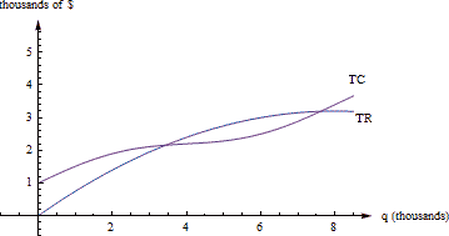
\includegraphics[width=0.4\textwidth]{img/chap2/image035.png}
    \caption{Total Revenue ($TR$) and Total Cost ($TC$) versus $q$ items.}
    \label{fig:2-3-trandtc}
\end{figure}
First, notice how to find the fixed cost and variable cost from the graph here. The fixed cost, $FC$, is the $y$-intercept of the $TC$ graph. ($FC=C(0)$.) The graph of variable costs would have the same shape as the graph of $TC$, shifted down.

Marginal cost for $q$ items is $MC(q)=C(q+1)-C(q)$, but that's impossible to read on this graph. How could you distinguish between $C(4022)$ and $C(4023)$? On this graph, that interval is too small to see, and our best guess at the secant line is actually the tangent line to the $TC$ curve at that point. (This is the reason we want to have the derivative definition handy.)
\begin{itemize}[label={}]
    \item $MC(q)$ is the slope of the tangent line to the $TC$ curve at the point $(q, C(q))$.
    \item $MR(q)$ is the slope of the tangent line to the $TR$ curve at the point $(q, R(q))$.
\end{itemize}
Profit is the distance between the $TR$ and $TC$ curves. If you experiment with a clear ruler, you'll see that the biggest profit occurs exactly when the tangent lines to the $TR$ and $TC$ curves are parallel. This is the rule that profit is maximized when $MR=MC$ which we'll explore in Section \ref{sec:app-opt}.

\begin{example}
Suppose the demand for widgets is $D(p)=\frac{1}{p}$, where $D$ is the quantity of widgets, in thousands, at a price of $p$ dollars. Approximate and interpret the derivative of $D$ at $p=\$3$.

\begin{solution} We can approximate $D'(3)$ by looking at a table, Table \ref{tab:2-3-Dprime}, of secant line slopes through the points $(3, D(3)) = \left(3, \frac{1}{3}\right)$ and $(3+\Delta p, D(3+\Delta p))$, where $\Delta p$ gets closer to $0$.

\begin{table}[ht!]
\begin{centering}
\begin{tabular}{lll}
\toprule
$\Delta p$ & $D(3+\Delta p)$ & $\dfrac{D(3+\Delta p)-D(3)}{\Delta p}$ \\
\midrule
1        & $\dfrac{1\mathstrut}{3+1\mathstrut} = 0.25$                & $\dfrac{D(4)     -D(3)}{1}     \approx -0.083333$ \\
0.1      & $\dfrac{1\mathstrut}{3+0.1\mathstrut} \approx 0.322581$    & $\dfrac{D(3.1)   -D(3)}{0.1}   \approx -0.107527$ \\
0.01     & $\dfrac{1\mathstrut}{3+0.01\mathstrut} \approx 0.332226$   & $\dfrac{D(3.01)  -D(3)}{0.01}  \approx -0.110742$ \\
0.001    & $\dfrac{1\mathstrut}{3+0.001\mathstrut} \approx 0.333222$  & $\dfrac{D(3.001) -D(3)}{0.001} \approx -0.111074$ \\
0.0001   & $\dfrac{1\mathstrut}{3+0.0001\mathstrut} \approx 0.333322$ & $\dfrac{D(3.0001)-D(3)}{0.0001}\approx -0.111107$ \\
\bottomrule
\end{tabular}
\caption{Average rate of change of demand approaching $D'(3)$.}
\label{tab:2-3-Dprime}
\end{centering}
\end{table}
Based on this, the quantities in the last column appear to be approaching $-0.1111\ldots$, which is $-\frac{1}{9}$. Later, we will show that that is indeed true. Since $D(p)$ has units ``thousands of widgets'' and the units for $p$ is ``dollars,'' the units for $D'(3)$ will be thousands of widgets per dollar. Therefore, $D'(3) \approx -0.111$ thousand widgets per dollar, or $-111$ widgets per dollar. This shows how the demand for widgets will change as the price increases.

Specifically, $D'(3)\approx -111$ widgets per dollar tells us that when the price of a widget is $\$3$, then the demand for widgets will decrease by about 111 widgets for every dollar the price increases.
\end{solution}\end{example} 

In the next section, we will lay the theoretical foundation to establish a rigorous and precise definition of the derivative of a function.


